\documentclass{article}
\usepackage[utf8]{inputenc}
\usepackage{graphicx}
\usepackage[%  
    pdfborder={0 0 0},
    linkcolor=black
]{hyperref}
\graphicspath{ {./images/} }
\setlength{\parindent}{0em}

\title{Relazione Progetto \\ Sistemi Operativi e Laboratorio}
\date{Luglio 2021}
\author{Samuele Calugi\\ Corso A \\ 579086}
\begin{document}
\maketitle
\tableofcontents

\section{Introduzione}
Come previsto dalle indicazioni dell'esame, il progetto di seguito è stato sviluppato nella versione ridotta e semplificata poiché la parte facoltativa non è 
prevista nell'appello di Luglio 2021. Il codice sorgente e i vari file necessari per il corretto funzionamento del programma sono stati caricati in una repository
pubblica su Github. È possibile accedere alla repository del progetto attraverso il seguente link: \url{https://github.com/Walrus98/Progetto-SOL}, così da poter 
visualizzare il codice sorgente e tutti i commit effettuati. \\ Le librerie utilizzate nel progetto sono le seguenti:
\begin{itemize}
    \itemsep 0em 
    \item \textbf{icl\_hash.h}, libreria vista a lezione utilizzata per la creazione di mappe.
    \item \textbf{list\_utils.h}, libreria realizzata dal sottoscritto utilizzata per la creazione di liste monodirezionali.
\end{itemize}

\subsection{Makefile}
L'intero progetto può essere compilato ed eseguito attraverso le seguenti regole:

\begin{itemize}
    \itemsep 0em 
    \item \textbf{all}: viene chiamato per default dal comando \textbf{make}, compila il client e il server attraverso le regole \textbf{build-client} e \textbf{build-server}. 
    \item \textbf{build-client}: compila tutti i file del client e genera l'eseguile.
    \item \textbf{build-server}: compila tutti i file del server e genera l'eseguile.
    \item \textbf{build-server-test1}: compila tutti i file del server con i config richiesti da test1 e genera l'eseguile.
    \item \textbf{build-server-test2}: compila tutti i file del server con i config richiesti da test2 e genera l'eseguile.
    \item \textbf{client}: esegue un clear della console e successivamente avvia il client con valgrind.
    \item \textbf{server}: esegue un clear della console e successivamente avvia il server con valgrind.
    \item \textbf{server-test1}: esegue un clear della console e successivamente avvia il server con i config richiesti da test1 con valgrind.
    \item \textbf{server-test2}: esegue un clear della console e successivamente avvia il server con i config richiesti da test2 con valgrind.
    \item \textbf{clean}: rimuove tutti i file object generati dalle regole elencate precedentemente.
\end{itemize}

\subsection{Test case}
Nel progetto è presente una cartella di nome \textit{"tests"} che al suo interno contiene i due file bash richiesti per testare il corretto
funzionamento del programma. I due script una volta avviati compilano in maniera autonoma client e server tramite le regole del Makefile sopra citate. Successivamente,
in base al tipo di file bash avviato, viene eseguito il server con il propio file config opportuno e un insieme di client che eseguono differenti richieste sul server.

\section{Funzionamento del programma}

\subsection{API}
Per potersi interfacciare con il server, il client include all'interno del suo codice un file header chiamato \textbf{client\_network.h}. Quest'ultimo possiede l'elenco di tutti i metodi
richiesti dal progetto dell'esame e permette quindi di per poter inviare e ricevere messaggi con il server attraverso l'utilizzo di un protocollo. Tutti i metodi del file header sono 
implementati nella classe \textbf{client\_network.c}.

\subsection{Protocollo}
I messaggi trasmessi dal client al server sono formati da due parti:
\begin{itemize}
    \itemsep 0em 
    \item \textbf{Header}, contiene un id che identifica il tipo di pacchetto trasmesso e la dimensione del payload.
    \item \textbf{Payload}, il contenuto effettivo del pacchetto che si vuole trasmettere.
\end{itemize}

Di conseguenza, ogni pacchetto è formato da due buffer: il \textbf{BufferHeader} e il \textbf{BufferPayload}.
\medskip 

Il \textbf{BufferHeader} ha dimensione fissa di \textbf{8 Byte} di cui:
\begin{itemize}
    \itemsep 0em 
    \item i primi 4 byte, (quindi il primo intero) contengono l'id del pacchetto che si vuole trasmettere.
    \item i 4 byte successivi, (quindi il secondo intero) contengono la dimensione del payload.
\end{itemize}

Il \textbf{BufferPayload} ha una dimensione variabile e contiene tutti i dati che si vogliono trasmettere

\begin{center}
    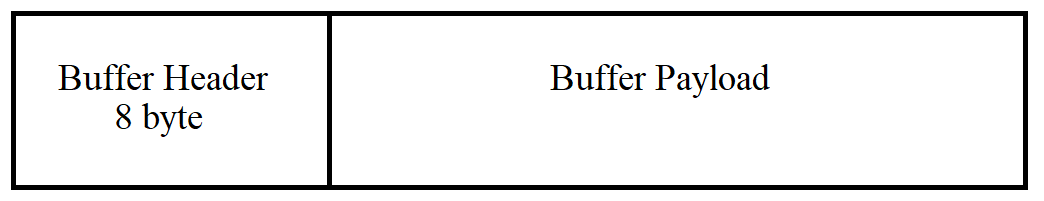
\includegraphics[width=\textwidth]{buffer}   
    Figure 1: Stuttura del buffer di invio di messaggi al server
\end{center}

Poichè il client ogni volta che invia un messaggio al server si mette in attesa di ricevere un messaggio di risposta da quest'ultimo (quindi i pacchetti da parte del 
client vengono inviati in maniera sequenziale), il server non ha bisogno di inviare al client l'id del pacchetto perché il client conosce già il tipo di pacchetto 
che sta per ricevere. Di conseguenza, il server invia prima la dimensione del pacchetto, poi il contenuto del buffer che vuole inviare. \\ In alcuni casi, se il server
non deve inviare nessun dato se non l'esito della richiesta che il client ha inviato, il server invia semplicemente un intero come messaggio di risposta:
nel caso di successo, il server invia 0, in caso di errore un numero negativo. 

\subsection{Server}

\subsection{Client}


\end{document}